\section{Natural Language Processing}

An inherent disparity between the languages used and understood by human beings
and those which are interpreted by machines introduces the requirement for a
system which is able to provide a form of compatibility between the two. Natural
language can be described as  a system of communication that has not consciously
been invented \citep{collins04} and typical examples of this are the languages
used by human beings to communicate with each other. English and Korean are two
such examples of natural languages and these evolve over time as words are added
and removed and the rules that define the language are refined or adapted,
meaning there is no immutable grammar for the language.

Conversely, formal (or artificial) languages are those which have been
fabricated for a specific purpose, and can be described using precise and
unambiguous mathematical rules \citep{jiang10}. An example of such a
mathematical rule is the Backus–Naur Form (BNF) grammar. Programming languages
such as Java or Python are examples of artificial languages, as these have been
created with a specific purpose in mind. The vocabularies of these languages are
well defined and free from ambiguities, making interpretation by the language’s
corresponding compiler a ‘black or white’ task where the given language to
compile is either valid or invalid.

Natural language processing (NLP) allows for the manipulation of natural
languages by a computational device \citep{bird09} and there are a number of
identified steps of the NLP process which have been developed, from scanning and
parsing, to meaning extraction and integration. In the context of solving
cryptic crosswords, a given clue would need to be broken down into meaningful
components which would allow, as an example, the word play and the definition
components to be identified and passed forward to the appropriate algorithms to
identify the correct answer.

\begin{figure}[H]
	\centering
	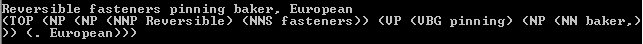
\includegraphics[width=\linewidth]{parse_tree.png}
	\caption{Creating a parse tree for a given sentence}
\end{figure}

\begin{flushright}
	\citep{halpern13}
\end{flushright}

\newpage
\subsection{The Steps of Natural Language Processing}

\subsubsection{Scanning}

A number of steps are typically involved in the processing of a natural
language. Assuming the input format of the natural language is in a textual form
as sentences (rather than as speech or handwriting); these chains of text may be
broken down into their separate components - the words which make up the
sentences. This process is known as scanning, and may itself comprise of several
sub-steps. The first step could likely involve breaking down the given textual
input into separate sentences \citep{apache13}.

\begin{figure}[H]
	\centering
	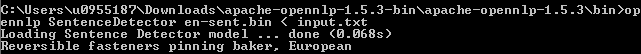
\includegraphics[width=\linewidth]{scanning.png}
	\caption{A single sentence is already in the desired state}
\end{figure}

Once the separation of any sentences present in the input has occurred, these
can be further divided into the separate words to achieve an array-like data
structure, such as [“\emph{Reversible}”, “\emph{fasteners}”, “\emph{pinning}”,
“\emph{baker}”, “\emph{European}”], a process which is referred to as
tokenising. It is important to consider the inclusion and placement of any
punctuation provided in the input text, as this may provide some indication as
to the separation of the cryptic crossword components  and increase the chances
of successfully calculating the answer. In the example provided, European
corresponds to the definition component of the clue, where Reversible fasteners
pinning baker relates to the word play component. Both components have been
clearly separated by a comma, though not all cryptic clues are presented in this
fashion.

\subsubsection{Parsing}

Parsing is a process used to ensure that a given sentence conforms to a grammar
and thus showing that it is syntactically correct \citep{mccluskey99}, and this
process can be demonstrated by creating a parse tree to represent the structure
of a given sentence. It may become apparent when attempting to solve the clues
of a cryptic crossword that certain elements of the provided clue sentences bear
some relation to the correct answer. To give an example, it may prove more
likely that the adjectives or verbs present in the input are synonyms of the
correct answer, where there may be little probability that the answer stems from
a synonym of any present determiners (the, this, a, some) or prepositions (on,
beneath, over, under). Likewise, adjectives or adverbs that hint at a particular
action such as \emph{reversible} or \emph{backwards} could reveal themselves as
more likely to be indicators that describe in what way the clue should be
manipulated.

\subsubsection{Referencing}

The ambiguous nature of cryptic clues may not allow for a straightforward parse
of an already ambiguous (natural) language, possibly contributing to the
complexity of the process of solving. It may be the case that multiple parses of
the same clue have to be taken forward to be processed before the solution can
be found. Once a parse tree has been selected for the given input, a number of
steps can be performed, which attempt to reduce the level of ambiguity. Lee
McCluskey outlines four methods which can be applied to achieve this:

\begin{itemize}
	\item \textbf{Contextual Disambiguation:} Such as referring to segments of
	a previous piece of text. Fred Bloggs may have been declared in a previous
	sentence, and from that point referred to as he.
	\item \textbf{Physical Constraints:} This refers to the literal meaning of
	a sentence of phrase, and uses known facts to assist in the reduction of
	ambiguity. The phrase “I answered the door in my pyjamas” could be taken to
	mean that the subject was either wearing their pyjamas when they answered
	the door, or that the door was wearing the subject’s pyjamas when they
	answered it. As it is unlikely that the door was physically wearing
	pyjamas, the parse suggesting this could be disregarded.
	\item \textbf{Default Roles in Known Verb Structures:} Some verbs may only
	be applied to a subset of subjects in order to make reasonable sense. In
	the example sentence “fruit flies like a banana”, one parse may take fruit
	as the noun, and flies as the verb. In this scenario, fruit	is physically
	incapable of flying, and so an alternative parse which taken “fruit flies”
	as the noun-phrase is more likely to be the correct parse of the sentence.
	\item \textbf{General Defaults:} To say that one is going to visit an old
	friend may imply that the friend has been known for a long time, or that
	the friend is of old age. While the correct interpretation may be context
	specific, the likelihood is that one particular interpretation will hold
	precedence over another. In this case, the friend is likely to have been
	known for a long time.
\end{itemize}

\begin{flushright}
	\citep{mccluskey99}
\end{flushright}

A parsing algorithm is used to obtain a complete parse tree for a given
sentence, providing insight into the complete structure of the sentences. It is
possible that this may not be required for the task at hand; a full parse may
provide more information than what is required to solve a cryptic clue. An
alternative mechanism exists, chunking, which may also be referred to as
\emph{light parsing}. This technique divides a sentence into a series of non-
overlapping chunks of text, which provide an overview of the input sentence
\citep{litman03}. One of the major benefits of this technique is the removal of
the need to resolve ambiguity, as chunks of the sentence are non-recursive,
unlike parsing which produces components of a sentence which may be nested in
each other.

\begin{figure}[H]
	\centering
	
\includegraphics[width=\linewidth]{pos_tagging.png}
	\caption{Assigning \emph{Parts of Speech} tokens to an input sentence}
\end{figure}

\subsubsection{Meaning Extraction}

Meaning extraction refers to the process of taking the parse and storing it in a
way which accurately represents the information it models \citep{mccluskey99}.
For example, the following cryptic crossword clues all map to the same answer,
and whilst they are written differently, they each imply the same meaning of
\emph{DRILL}:

\begin{itemize}
	\item \emph{Doctor gives patients exercise}
	\item \emph{Doctor needing a doctor for practice}
	\item \emph{GP not fit for practice}
\end{itemize}

\begin{flushright}
	\citep{gordius03}
\end{flushright}

Effective meaning extraction will ensure that each distinct clue may help to
ensure that variations of the same will be mapped to a single, internal
representation and this will allow for the answer to be retrieved from a
database without having to recalculate what has already been processed once.

\subsection{Natural Language Processing Libraries}

There exists a range of NLP libraries that offer many natural language
processing functions for a variety of programming languages. Development on a
number of these libraries has become stale, and others are available only for
use after purchasing a commercial licence. Below are a selection of available
libraries which have recently been updated and are available under some form of
free software licence.

\begin{table}[H]
	\centering
	\small
	\begin{tabular}{|p{3.3cm}|p{4.9cm}|p{3.0cm}|p{2.3cm}|}
	\hline
	\textbf{Library} & \textbf{Licence} & \textbf{Last Updated}  &
	\textbf{Supported Languages} \\ \hline
	OpenNLP & Apache 2.0 &  April 2013 & Java \\ \hline
	NLTK & Apache 2.0 & November 2012 & Python \\ \hline
	Stanford CoreNLP & GNU General Public Licence & June 2013 & Java \\	\hline
	\end{tabular}
	\caption {A comparison of available NLP libraries}
\end{table}

\subsubsection{OpenNLP}

OpenNLP provides the ability to carry out a range of natural language processing
functions, including parsing, chunking and name finding, where the latter aims
to recognise proper nouns in specified text such as person names. The features
of the library utilise a maximum entropy model, and this allows the performance
of the software to be enhanced as it uses training data to learn
\citep{apache13}. This allows for each component of the toolkit to refine as the
subset of training data increases over time, with the aim of increasing the
accuracy of the corresponding NLP component. The library is available for use in
a Java environment or can be accessed directly through a command line interface,
but the general usage of the library requires providing an applicable model and
language data as input, for which the model will be utilised for the language
processing.

\paragraph{Models}

A number of models are provided for use with the NLP library. These include, but
are not limited to, models to assist in the process of parsing, chunking and
detecting sentences. A number of libraries also exist which allow for the
identification of person names, company names, times, dates or location in input
text. These existing models may be further trained in a bid to increase their
effectiveness.

\paragraph{DocumentCategoriser}

Another prominent feature of the library is the ability to classify input text
into a range of predetermined categories using the aforementioned maximum
entropy model. Once a model has been created, which contains a series of example
inputs along with their corresponding categories, further inputs to the system
will be paired with a \emph{best outcome} classification.

\begin{figure}[H]
	\centering
	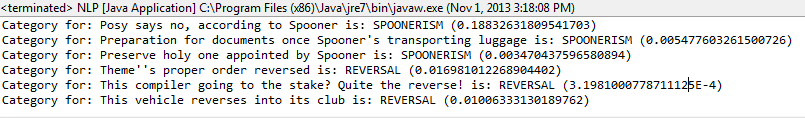
\includegraphics[width=\linewidth]{document_categoriser.png}
	\caption{A demonstration of the OpenNLP DocumentCategorizer}
\end{figure}

\subsubsection{NLTK}

The Natural Language Toolkit is an alternative library which exists with an
open-source licence variant. NLTK exists for use with the Python programming
language and possesses a similar infrastructure to OpenNLP, where trained models
are used to allow each component of the software package to function correctly
\citep{nltkproject12}. The package is supplemented by a comprehensive e-book,
detailing and providing examples of the usage of each component available.